\documentclass[a4j,11pt]{ltjsarticle}    % 文章クラスとオプション設定
%%%%%%%%%% スタイル %%%%%%%%%%%%%%%%%%%%%%%%%%%%%%%%%%%%%%%%%%%%%%%%%%%%%%%%%%%%%%%%%%%%%%%%%%%%%%

\usepackage{comment}    % 複数行コメント

% 余白の調整
\usepackage[top=30truemm,bottom=30truemm,left=20truemm,right=20truemm]{geometry}

% 数式関連
\usepackage{amsmath,amssymb,nccmath,siunitx}    % 数式
\usepackage{bm}         % ベクトルの太文字

% 画像関連
\usepackage{graphicx} % 画像

\usepackage{here}% figureの位置調整
% 表設定
\usepackage{multirow}   % 表の行の結合
\usepackage{longtable}  % ページをまたぐ長い表

\usepackage{url}

%%%%%%%%%% 本文 %%%%%%%%%%%%%%%%%%%%%%%%%%%%%%%%%%%%%%%%%%%%%%%%%%%%%%%%%%%%%%%%%%%%%%%%%%%%%%%%%

\begin{document}

% !TEX root = main.tex

%%%%%%%%%%%%%%%%%%%%%%%%%%%%%%%%%%%%%%%%%%%%%%%%%%%%%%%%%%%%%%%%%%%%%%%%%%%%%%%%%%%%%%%%%%%%%%%%

\title{RLC回路の過渡現象(後半)}
\author{}
\date{}
\maketitle

%%%%%%%%%%%%%%%%%%%%%%%%%%%%%%%%%%%%%%%%%%%%%%%%%%%%%%%%%%%%%%%%%%%%%%%%%%%%%%%%%%%%%%%%%%%%%%%%

% !TEX root = main.tex

%%%%%%%%%%%%%%%%%%%%%%%%%%%%%%%%%%%%%%%%%%%%%%%%%%%%%%%%%%%%%%%%%%%%%%%%%%%%%%%%%%%%%%%%%%%%%%%%
\section{目的}
%%%%%%%%%%%%%%%%%%%%%%%%%%%%%%%%%%%%%%%%%%%%%%%%%%%%%%%%%%%%%%%%%%%%%%%%%%%%%%%%%%%%%%%%%%%%%%%%

パルス大電流の取り扱い,及びそれを利用したLCR回路の過渡現象を理解する.

% !TEX root = main.tex

%%%%%%%%%%%%%%%%%%%%%%%%%%%%%%%%%%%%%%%%%%%%%%%%%%%%%%%%%%%%%%%%%%%%%%%%%%%%%%%%%%%%%%%%%%%%%%%%
\section{原理}
%%%%%%%%%%%%%%%%%%%%%%%%%%%%%%%%%%%%%%%%%%%%%%%%%%%%%%%%%%%%%%%%%%%%%%%%%%%%%%%%%%%%%%%%%%%%%%%%

\subsection{コンデンサ放電}
大電流をソレノイド$L$に流すことで強い磁場$B$を発生させる.
このためには大きな電流$I$が必要となり,本実験ではコンデンサ放電を用いる.
コンデンサ放電では,コンデンサ$C$を高電圧で充電することにより大電荷$Q$
を貯めることができ,この$Q$を急速放電$\left(\frac{d}{d t} \gg 1\right)$
させることで,$\frac{d Q}{d t}=I$により大きな$I$を発生させる.

\subsection{RLC回路における過渡現象の原理}
キルヒホッフの第2法則よりRLC回路では以下の回路方程式が成り立つ.
$$
R i+L\frac{di}{dt}+\frac{1}{c} \int i d t=E
$$
ここで,$D=\left(\frac{R}{2 L}\right)^2-\frac{1}{L C}, \alpha=-\frac{R}{2 L} , \beta=\sqrt{\left(\frac{R}{2 L}\right)^2-\frac{1}{L C}}, \beta^{\prime}=\sqrt{-\left\{\left(\frac{R}{2 L}\right)^2-\frac{1}{L C}\right\}}$
とおくと,電流 $i$ は以下の式で描かれる.
$$
\begin{gathered}
\mathrm{D}>0 \text { のとき } i=\frac{E}{\beta L} e^{\alpha t} \sinh \beta t \\
\mathrm{D}<0 \text { のとき } i=\frac{E}{\beta^{\prime} L} e^{\alpha t} \sinh \beta^{\prime} t \\
\mathrm{D}=0 \text { のとき } i=\frac{E}{L} e^{\alpha t}
\end{gathered}
$$
このとき,電流$i$は$D>0$のとき過減衰,$D=0$のとき臨界減衰,$D<0$ のとき不足減衰
となる.



% !TEX root = main.tex

%%%%%%%%%%%%%%%%%%%%%%%%%%%%%%%%%%%%%%%%%%%%%%%%%%%%%%%%%%%%%%%%%%%%%%%%%%%%%%%%%%%%%%%%%%%%%%%%
\section{実験}
%%%%%%%%%%%%%%%%%%%%%%%%%%%%%%%%%%%%%%%%%%%%%%%%%%%%%%%%%%%%%%%%%%%%%%%%%%%%%%%%%%%%%%%%%%%%%%%%

\subsection{実験器具}
TEKTRONIX TBS1022 オシロスコープ,ソレノイドコイル,高電圧パルス大電流発生
電源,セメント抵抗$(1\Omega)$,可変抵抗$(<20\Omega)$

\newpage

\subsection{実験方法}
\subsubsection{セットアップ}
\begin{enumerate}
    \item 図1のように回路を作成する.
    \item 充電電圧調整ダイアルがゼロになっていることを確認してから,
    パルス電源の電源スイッチをONにする.
    \item 電圧調整ダイアルをゆっくりと回し,充電電圧を調整する.
    本実験では,$50\,\si{\volt}$以下の電圧で行う.
    \begin{figure}[H]
        \begin{center}
            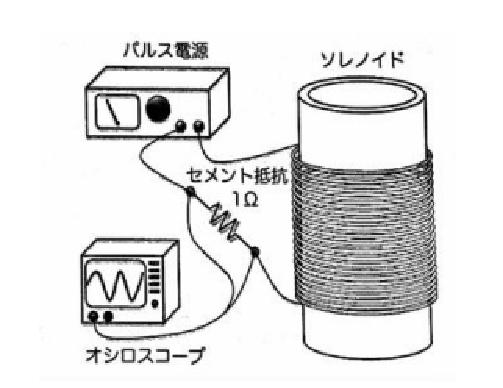
\includegraphics[scale=0.75]{figure1.pdf}
            \caption{実験装置}
        \end{center}
    \end{figure}
\end{enumerate}

\subsubsection{$L$の測定}
図1に示す実験配置において,パルス電流を流した際にセメント抵抗$(1\,\Omega)$の両端
にかかる電圧波形を記録する.ただし,パルス電源内には,$12\,\si{\mu F}$のコンデンサ
が入っており,$L$の計算を行う際には,セメント抵抗の抵抗値$(1\,\Omega)$は無視して
良いとする.さらに,電圧波形から周期$T$を測定することで,ソレノイドのインダクタンス
$L$の値を算出する.このときインダクタ$L$は,以下の式で算出される.
$$
L=\frac{r^2}{4\pi^2C}
$$


\subsubsection{$R$の決定}
実験課題1から算出したインダクタンス$L$の値を用いて,電流波形が臨界制動波形となる
際の$R$の値を計算し,実際にその抵抗$R$を回路に接続することで電流波形が
臨界制動波形となることを確認し,記録する.
このとき,抵抗値$R$は以下の式で算出される.
$$
R^2=\frac{4L}{C}
$$
% !TEX root = main.tex

%%%%%%%%%%%%%%%%%%%%%%%%%%%%%%%%%%%%%%%%%%%%%%%%%%%%%%%%%%%%%%%%%%%%%%%%%%%%%%%%%%%%%%%%%%%%%%%%
\section{結果}
%%%%%%%%%%%%%%%%%%%%%%%%%%%%%%%%%%%%%%%%%%%%%%%%%%%%%%%%%%%%%%%%%%%%%%%%%%%%%%%%%%%%%%%%%%%%%%%%


% !TEX root = main.tex

%%%%%%%%%%%%%%%%%%%%%%%%%%%%%%%%%%%%%%%%%%%%%%%%%%%%%%%%%%%%%%%%%%%%%%%%%%%%%%%%%%%%%%%%%%%%%%%%
\section{データ解析と考察}
%%%%%%%%%%%%%%%%%%%%%%%%%%%%%%%%%%%%%%%%%%%%%%%%%%%%%%%%%%%%%%%%%%%%%%%%%%%%%%%%%%%%%%%%%%%%%%%%
\begin{enumerate}
    \item 実験課題1で得られた$L$の実験値を理論値と比較せよ.
    なお,計算においては長岡係数を考慮すること.
    \begin{description}
        \item[] 
    \end{description}

    \item (1)で計算した$L$の理論値を用いて,臨界制動となるときの$R$の値を算出
    せよ.また,実験的に求めた$R$の値と比較し,$R$の値が異なるときは,その原因
    を考察せよ.
    \begin{description}
        \item[] 
    \end{description}
\end{enumerate}
% !TEX root = main.tex

%%%%%%%%%%%%%%%%%%%%%%%%%%%%%%%%%%%%%%%%%%%%%%%%%%%%%%%%%%%%%%%%%%%%%%%%%%%%%%%%%%%%%%%%%%%%%%%%
\section{宿題}
%%%%%%%%%%%%%%%%%%%%%%%%%%%%%%%%%%%%%%%%%%%%%%%%%%%%%%%%%%%%%%%%%%%%%%%%%%%%%%%%%%%%%%%%%%%%%%%%

\begin{enumerate}
    \item サイリスタ(SCR)の動作原理を調べよ.
    \begin{description}
        \item[] 
    \end{description}
\end{enumerate}

%%%%%%%%%% 参考文献 %%%%%%%%%%%%%%%%%%%%%%%%%%%%%%%%%%%%%%%%%%%%%%%%%%%%%%%%%%%%%%%%%%%%%%%%%%%%%%

% !TEX root = main.tex

%%%%%%%%%% 参考文献 %%%%%%%%%%%%%%%%%%%%%%%%%%%%%%%%%%%%%%%%%%%%%%%%%%%
\begin{thebibliography}{99}
    \newcounter{num}
    \setcounter{num}{2}
    \bibitem{電子システム工学基礎実験テキスト}
\end{thebibliography}

\end{document}